\documentclass[../p051main.tex]{subfiles}
\graphicspath{{\subfix{../figures/}}}

\begin{document}

\chapter{Optics}
\section{Light and Materials}
Now we'll turn our attention to a study of light in its own right.
To begin, we'll need to modify Maxwell's equations a little bit.
Recall that they were constructed in free space, so in order to make them valid in materials we must substitute $\epsilon_0 \to \kappa_E \epsilon_0$ and $\mu_0 \to \kappa_B \mu_0$.
Consequentially, in matter we have the wave equation
\[ \nabla^{2} \mathbf{E} = (\kappa_e \kappa_m) \mu_0 \varepsilon_0 \frac{\partial^{2} \mbf{E}}{\partial t^2}. \]
If we define the material's index of refraction $n = \sqrt{\kappa_e \kappa_m}$, then we find that light travels at
\[ v = \frac{1}{\sqrt{\kappa_e \kappa_m}} \frac{1}{\sqrt{\mu_0 \epsilon_0}} = \frac{c}{n} \]
when in a medium.
It follows that electromagnetic waves satisfy $B_0 = E_0 n / c$, and that their intensities are given by $I = E_0^2 n / 2\mu_0 c$.

A point at which materials with different refractive indices meet is called an interface.
When an electromagnetic wave is incident on an interface, it gets split into a reflected wave and a transmitted wave.
For normal incidence, the equations describing this split are
\begin{align*}      
    \mathbf{E}_i &= E_i \,\hat{y}\, \cos (k_1 x - \omega_1 t), & \mathbf{B}_i &= \frac{E_i n_1}{c} \,\hat{z}\, \cos (k_1 x - \omega_1 t), \\
    \mathbf{E}_r &= E_r \,\hat{y}\, \cos (-k_1 x - \omega_1 t), & \mathbf{B}_r &= \frac{E_r n_1}{c} \,(-\hat{z})\, \cos (-k_1 x - \omega_1 t), \\
    \mathbf{E}_t &= E_t \,\hat{y}\, \cos (k_2 x - \omega_2 t), & \mathbf{B}_t &= \frac{E_t n_2}{c} \,\hat{z}\, \cos (k_2 x - \omega_2 t),
\end{align*}
where $n_1$ is the refractive index of the first material and $n_2$ is that of the second.
We can relate all of these equations using Ampere's law and Faraday's law; if we take thin loops that are parallel to $\mbf{E}$ and $\mbf{B}$, respectively, we get
\[ \oint \mbf{E} \cdot d\mbf{l} = 0, \qquad \oint \mbf{B} \cdot d\mbf{l} = 0. \]
So if we have an interface at $x=0$, then the relationship between the electric fields is
\[ E_i \cos(-\omega_1 t) + E_r \cos(-\omega_1 t) - E_t \cos (-\omega_2 t) = 0. \]
The only way for this equation to be true for all $t$ is if $\omega_1 = \omega_2 - \omega$. meaning the frequency of light does not change in a medium!
All that changes, then, is the wavenumber $k = \omega / v = 2\pi n / \lambda_\textrm{vac}$.

Anyway, cancelling the cosines gives $E_i + E_r = E_t$.
A similar analysis for magnetic fields would give $E_i n_1 - E_r n_1 = E_t n_2$, and solving the resulting system of equations gives
\[ E_r = \left( \frac{n_1 - n_2}{n_1 + n_2} \right) E_i, \qquad E_t = \left( \frac{2n_1}{n_1 + n_2} \right) E_i.  \]
Note that $E_r$ is negative when $n_1 < n_2$, so in this case the reflected wave is out of phase with the transmitted wave.
Otherwise the waves are in phase.
Here's a handy mnemonic to keep track:
\begin{center}
    ``Low to high, add a $\pi$.'' \qquad ``High to low, let it go.''
\end{center}
For scenarios with multiple interfaces we simply apply these rules several times, often ignoring light that bounces back and forth between interfaces many times.

\section{Polarization}
The orientation of an electromagnetic wave, called its polarization, can be described entirely by the direction in which its electric field points.
Most common sources of light produce unpolarized light, in which the direction of $\mbf{E}$ is basically random and time-varying.
When light is polarized, though, it can come in three different forms: linear, circular, and elliptical.
\begin{itemize}
    \item For light that is linearly polarized, $\mbf{E}$ points in a constant direction as the wave propagates.
    A wave propagating in the $x$-direction may be polarized along $\hat y$, $\hat z$, or some linear combination of the two.

    \item Circularly polarized light is comprised of two identical components that are out of phase by precisely a quarter-cycle, so that the electric field appears to trace out a circle in space.
    Confusingly, optics people tend to specify the ``handedness'' of this tracing with respect to the receiving end of the light, so we point our thumb opposite the direction of propagation and curl our fingers in such a way that matches the twist of the $\mbf{E}$-field.
    This gives us the following parameterizations.
    \begin{align*}
        \textrm{RHCP: } \mathbf{E} &= E_0 \,\hat{y} \cos(kx - \omega t) + E_0 \,\hat{z} \sin(kx - \omega t) \\
        \textrm{LHCP: } \mathbf{E} &= E_0 \,\hat{y} \sin(kx - \omega t) - E_0 \,\hat{z} \cos(kx - \omega t)
    \end{align*}
    \vspace{-18pt}

    \item Elliptical polarization occurs we have two identical components that are out of phase by a different amount, so that the electric field appears to trace out an ellipse in space.
    Linear and circular polarization can be seen as special cases of elliptical polarization.
\end{itemize}
The polarization of light can be controlled using filters called polarizers.
In the case of a linear polarizer, the incident electric field is split into two components $\mbf{E}_\textrm{in} = \mbf{E}_\parallel + \mbf{E}_\perp$ which are parallel and perpendicular to the direction of polarization, respectively.
As $\mbf{E}_\textrm{in}$ passes through, $\mbf{E}_\parallel$ is transmitted entirely while $\mbf{E}_\perp$ is absorbed entirely.
So if $\mbf{E}_\textrm{in}$ is polarized at an angle $\theta$ with respect to the polarization direction, then $E_\textrm{out} = E_\textrm{in} \cos \theta$ and we have Malus's law
\[ I_\textrm{out} = I_\textrm{in} \cos^2 \theta. \]
Linear polarizers are the basis for a host of technologies, like polarizing sunglasses and LCD screens!
They also exhibit some strange behavior due to Malus's law.
Two polarizers oriented perpendicular to one another will block out all light, but if a third is added at a $45^\circ$ angle to both of them, then suddenly some light will pass through.

There are other ways light can be polarized, too.
One is through scattering: if some light traveling in the $\hat z$-direction and is incident on a collection of dust, then this dust is excited and begins to vibrate in the $xy$-plane (i.e., in the plane of the electromagnetic field).
When light is emitted its propagation direction and polarization direction both remain in this plane and, of course, are orthogonal to each other.

Polarization by reflection may also occur when light reflects on an interface between materials.
Define the light's plane of incidence to be that spanned by the vector normal to the interface and that which points in the direction of incident light.
For any interface, the incidence-plane component of the reflected electromagnetic wave is dependent not only on the materials' refraction indices, but also on the angle of incidence.
Thus there is a critical angle, called the Brewster's angle, such that all light polarized in the plane of incidence is transmitted.
(This also happens to be the angle at which the reflected and transmitted light are orthogonal to one other.)
As a result, the reflected light is polarized orthogonal to the plane of incidence.

Finally, polarization can occur when light passes through a birefringent material, the details of which don't concern us.
In the big picture, some materials have refractive indices that depend on the direction in which light propagates through them.
Such a material has an intrinsic optic axis with index $n_o$, while the perpendicular axis has $n_e$; the perpendicular components of the normally incident wave (the $o$- and $e$-rays) undergo a relative phase shift
\[ \Delta \phi = \frac{2\pi}{\lambda} (n_o - n_e)d, \]
where $\lambda$ is the light's wavelength and $d$ is the width of the material.
If $\Delta \phi = \pi / 4$ or a coterminal equivalent, then we have a quarter-wave plate that can be used to convert $45^\circ$-incident linearly polarized light into circularly polarized light, or vice versa.
In the case of $\Delta = \pi / 2$ we have a half-wave plate which ``mirrors'' the polarization of the incident light.

\section{The Photon}
In classical optics, light is comprised of electromagnetic waves and has intensity given by the electric field, vacuum permeability, and speed of light.
But we now know light to exhibit a kind of wave-particle duality---in quantum optics it is comprised of photons, each of which has an energy $E = h\nu$, where $\nu$ is the frequency of the light and $h$ is called Planck's constant.
So if a beam of $N$ photons is incident on an area $A$ in a time $\Delta t$, then the intensity of the light beam they comprise is given by
\[ I = \frac{N h\nu}{A\Delta t}. \]
The quantum nature of light has been experimentally verified several times using various experiments.
One examined the photoelectric effect, the observation that electromagnetic radiation can ``kick'' electrons off the surface of a metal.
These electrons leave the metal with, at most, a kinetic energy $K_\textrm{max} = h\nu - W$, where $W$ is the energy expended in escaping the metal to begin with, called the metal's work function.
In the historical experiment, the metal is the high-potential terminal of an uncharged parallel-plate capacitor held in a vacuum chamber.
This capacitor is part of a larger circuit so that, if the ejected electrons have a high enough kinetic energy, they can make it to the other side of the capacitor and drive a current.
The critical potential where no electrons make it to the other terminal is called the stopping potential $V_\textrm{stop}$, and we have
\[ q_e V = h\nu - W. \]
Experiments have verified this, meaning the stopping potential has absolutely nothing to do with the intensity of the incident light.
This opposes the classical theory that would have $V_\textrm{stop}$ increase with intensity.

In another experiment, high-energy light is scattered off of a graphite target.
Assuming light is quantized, we'll see a photon with wavelength $\lambda$ collide with an electron of mass $m_e$; the photon is deflected by an angle $\theta$ with a new wavelength $\lambda'$, while the electron is sent off at an angle $\phi$ with momentum $p_e$.
Using relativistic conservation of momentum and energy we get the equations
\begin{gather*}
    \frac{h}{\lambda} = \frac{h}{\lambda'} \cos \theta + p_e \cos \phi, \qquad 0 = \frac{h}{\lambda'} \sin \theta - p_e \sin \phi, \\
    m_e c^2 + \frac{hc}{\lambda} = \frac{hc}{\lambda'} + \left( p_e^2 c^2 + m_e^2c^4 \right)^{1/2}.
\end{gather*}
Solving this system would yield
\[ \lambda' - \lambda = \frac{h}{m_e c} (1 - \cos \theta) \]
which, again, is consistent with experiment.
This phenomenon is known as Compton scattering.
\vspace{1pt}

\parbox{0.65\textwidth}{
    At this point we're confident that light comes in discrete quanta, so we might wonder now how these quanta behave.
    We can investigate this using a Mach-Zehnder interferometer, illustrated at right.
    
    \vspace{6pt}
    Elements B and C are mirrors, while the semicircles are detectors.
    Elements A and D are beam splitters, which reflect half of any incident light and transmit the rest.
    If a single photon is incident, though, that photon doesn't get cut in half and take both paths; rather, it picks one path and sticks with it.
    This pick is random, too---there is no way to deterministically predict which way the photon will go.
    The best we can do is work in probabilities.

    \vspace{6pt}
    It \hfill turns \hfill out \hfill that \hfill these \hfill probabilities \hfill aren't \hfill as \hfill simple \hfill as \hfill flipping \hfill a \hfill coin
}\parbox{0.35\textwidth}{
    \quad\;
    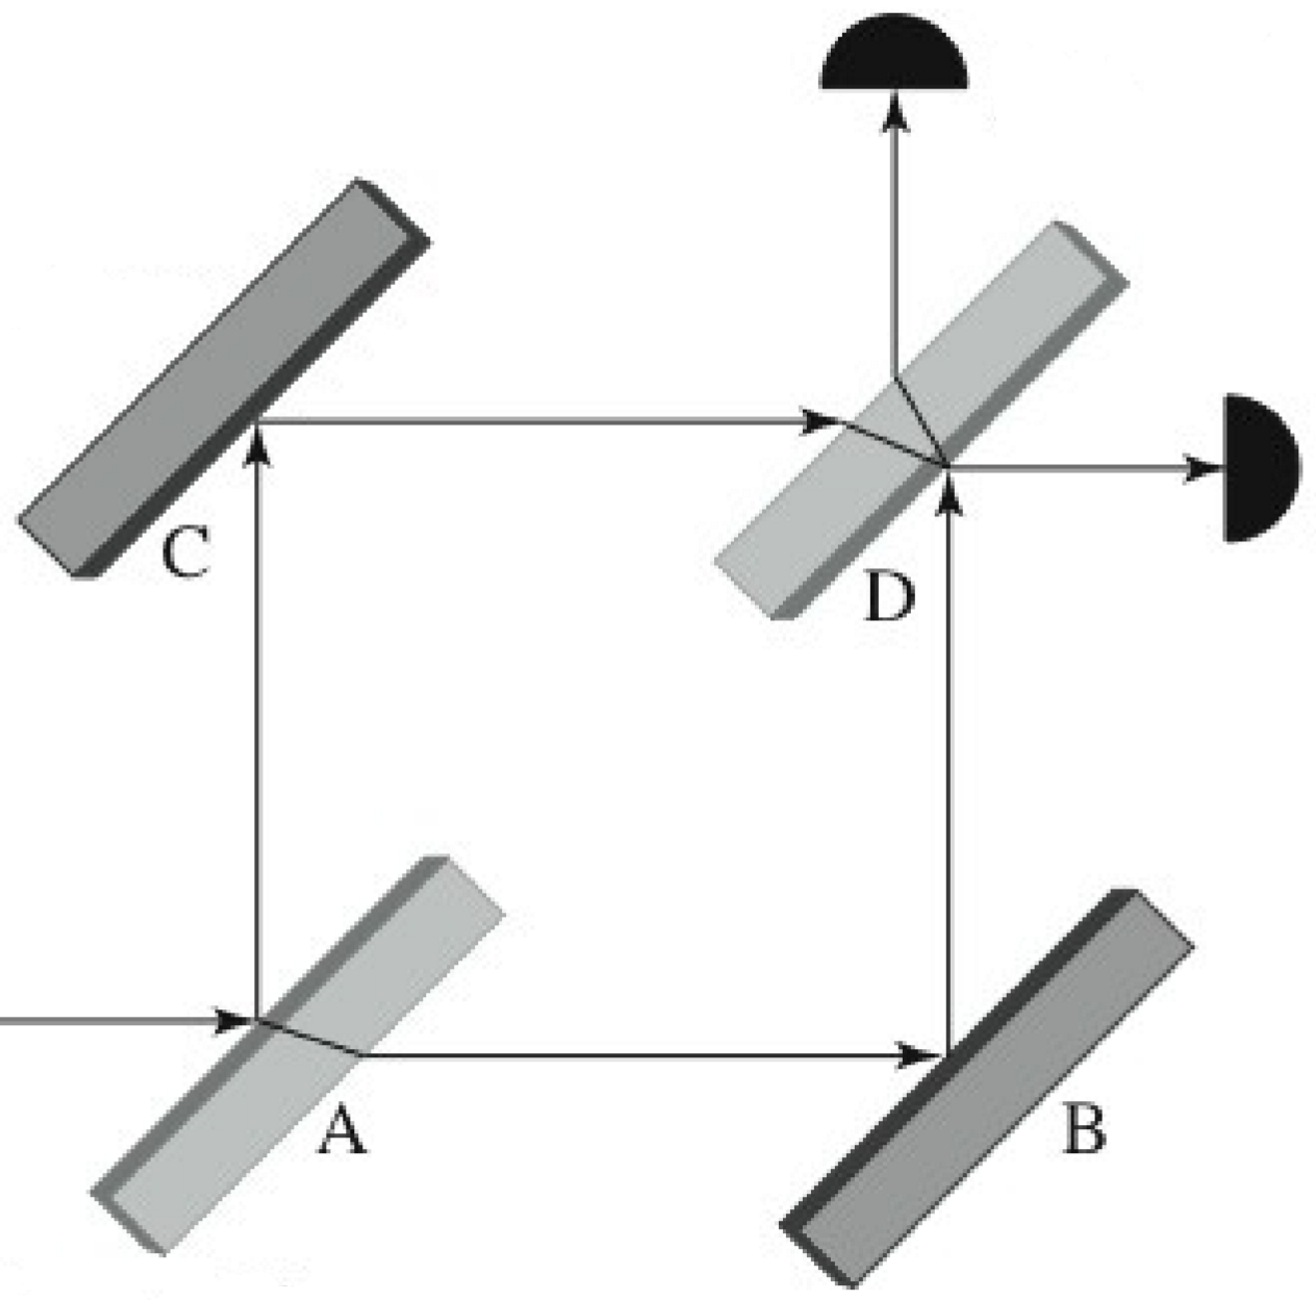
\includegraphics[width=0.3\textwidth]{machZehnder.png}
}

\vspace{-4pt}
for each splitter.
Assuming photons are sent into splitter A at a constant rate, experiments show that the rate at which either of the detectors receives photons varies sinusoidally with distance.
This suggests that the relevant quantity is not just a probability, but also an associated phase.
Complex numbers happen to describe this behavior in just the right way!

In our theory of quantum optics, each event has an associated complex number $z$ called a probability amplitude.
There are three fundamental rules that these probability amplitudes abide by, and they're surprisingly intuitive.
\begin{enumerate}
    \item If an event has probability amplitude $z$ with complex conjugate $z^*$, then the probability of the event occurring is given by
    \[ P = |z|^2 = z^*z. \]

    \item If an event can be broken down ito a series of steps, then its probability amplitude is the product of those for each step:
    \[ z = z_1 z_2 z_3 \cdots. \]

    \item If an event can happen in multiple independent ways, then its probability amplitude is the sum of those for each way:
    \[ z = z_1 + z_2 + z_3 + \cdots. \]
\end{enumerate}
Below is a table of probability amplitudes for some events that are relevant to our discussion.
\begin{center}
    \def\arraystretch{1.3}
    \begin{tabular}{c|c}
        Event & Amplitude \\ \hline
        travel & $z = e^{ikd}, \;k = 2\pi n / \lambda$ \\
        transmission & $z = \sqrt{P_\textrm{trans}}$ \\
        reflection & $z = \pm \sqrt{P_\textrm{ref}}$
    \end{tabular}
\end{center}
Here $d$ is the distance a photon travels in a medium with refractive index $n$.
(Note that $n = 1$ for a vacuum.)
The probability amplitude for photon reflection has a $\pm$ to account for the phase shift that occurs at interfaces with higher-index materials.

\section{Multiple-slit Diffraction}
Consider a laser that shines through two very narrow slits and onto a faraway wall.
On the wall we may expect to see two bright peaks of light, but instead there's a row of bright bands that peak right between the slits.
There are both classical and quantum explanations for this phenomenon; we will, of course, focus on the quantum one here.

There are two paths light can take to get to any given point on the wall, one for each slit.
Let $d$ be the small distance between the slits, $d_0$ the distance from the laser to the slits, and $d_1, d_2$ the distances from each slit to the wall.
So we have the probability amplitudes
\[ z_1 = e^{ikd_0} r e^{ikd_1} \quad\textrm{and}\quad z_2 = e^{ikd_0} r e^{ikd_2}, \]
where $r$ is the probability amplitude of the light going in the proper direction to reach the point on the wall.
(Strictly speaking $r$ depends on the deflection angle $\theta$, which is different for the two slits.
The difference is so slight, though, that they're approximately equal.)
Adding these amplitudes gives
\[ z = z_1 + z_2 = r e^{ikd_0} e^{ikd_1} \left( 1 + e^{ik(d_2 - d_1)} \right), \]
and the probability
\[ P = 4r^2 \cos^2 \left( \frac{k(d_2-d_1)}{2} \right). \]
If the wall is very far away then we have $d_2 - d_1 = d \sin \theta$ and
\[ P = 4r^2 \cos^2 \left( \frac{kd\sin \theta}{2} \right) = 4r^2 \cos^2 \left( \frac{\pi d \sin \theta}{\lambda} \right). \]
Notice that this probability is maximized when the phase difference $kd \sin \theta$ is an integer, so that the each slit produces light perfectly in phase.
Similarly, the probability is minimized when the phase difference is at midpoints between integers.
Thus we see
\[ \textrm{maxima at } d \sin \theta = 0\lambda,\, 1\lambda,\, 2\lambda,\, \ldots \quad\textrm{ and }\quad \textrm{minima at } d \sin \theta = \frac{1}{2}\lambda,\, \frac{3}{2}\lambda,\, \frac{5}{3}\lambda,\, \ldots\,. \]
As we increase the number of slits, the width of each bright spot decreases to a point.
This is because, as we increase the number of slits, there are more values of $\theta$ that can cause destructive interference.
To see this, note how the probability for $n$ slits is given by
\[ P = r e^{ikd_0} e^{ikd_1} \left( 1 + e^{i\theta} + e^{i(2\theta)} + \cdots + e^{i(n\theta)} \right). \]
We might model each slit's complex exponential as a phasor, and that all of these phasors are being summed to get the total probability for a point on the wall.
If for a particular $\theta$ the phasors sum to zero (which manifests itself in phasor space as a regular $n$-gon), then there will be perfect destructive interference there.

\section{Single-slit Diffraction}
Now suppose that, instead of being faced with a row of infinitesimal slits, we have a single slit of finite width $a$ that is parallel with a faraway wall.
Suddenly, the path of an incident photon can no longer be entirely described by its angle of deflection!

Consider an infinitesimal bit $dx$ of the slit, located a distance $x$ from one of its edges.
The probability amplitude associated with a photon passing through this bit and landing on a particular spot on the wall is
\[ dz = dr \,e^{ik(d_1 + x \sin \theta)}, \]
where $d_1$ is the distance between the edge of the slit and the spot on the wall, $\theta$ is the direction in which a photon must be deflected to hit this spot, and $dr$ is the probability amplitude associated with this deflection.

The probability amplitude for the entire slit is the integral of $dz$ over the entire slit.
We'll take $dr = (r / a) dx$ in order to normalize our probabilities (where we've assumed that $dr$ is independent of where we are on the slit), so we have
\[ z = \int_{0}^{a} \frac{r}{a} dx \,e^{ik(d_1 + \sin\theta)} = \frac{r e^{ik(d_1 + (a/2)\sin \theta)}}{ika\sin \theta} \left( e^{\frac{1}{2}ika\sin \theta} - e^{-\frac{1}{2}ika\sin \theta} \right) = \frac{r e^{i(\cdots)}}{\frac{ka}{2}\sin \theta} \sin \left( \frac{ka}{2}\sin \theta \right). \]
Defining $\alpha = (ka / 2)\sin \theta$ gives
\[ P = \frac{r^2}{\alpha^2} \sin^2 \alpha. \]
On our faraway wall we would see one bright peak at the center of the slit, and then a bunch of much dimmer peaks going off to the side.
(About ninety percent of the intensity of the light is concentrated within this central bump.)
We see perfect destructive interference at integer multiples of $\pi$ for $\alpha$, meaning the first minima $\pm\theta_1$ occur where $\sin\theta_1 = \lambda / a$.

This actually gives us a criterion for determining whether or not two objects, say headlights on a car, are distinguishable from a distance!
Specifically, according to the Rayleigh criterion two objects are ``barely resolvable'' when the center of one diffraction pattern is at the minimum of the other.
Any closer and they mesh together into one.

Now, in this entire discussion of quantum optics we've ignored one glaring issue: for any point in space, there's actually an infinite number of paths a photon can take to get there!
There's no obvious reason light should prefer traveling in straight lines over, anything else.
The principle of least time resolves this issue: if there is a continuous range of paths that light can take between two points in space, the only path that contributes significantly to the probability of detection at the end point is that of minimum time (or, more importantly, minimum phase).
At a high level, this is because the shorter paths are only marginally different in phase and so tend to constructively interfere, while longer paths are quite different from one another and tend to cancel one another out.

Finally, we cap everything off with one more disturbing revelation.
Everything we've just discussed--diffraction, interference, all that--also works with massive particles like helium atoms.
This strongly suggests that matter, too, has wave-like properties that can be described in terms of probability amplitudes.
We might make a leap in logic and define the (nonrelativistic) de Broglie wavelength
\[ \lambda_\textrm{dB} = \frac{h}{mv}, \]
inspired by how $E = h\nu = pc$ for a photon, meaning it has $\lambda = h / p$.
In principle every bit of matter has a de Broglie wavelength, but at the macroscopic level the wavelengths are far too small relative to the apertures we face in real life to cause any diffraction.
Despite that oddity, this leap is a good one, and it turns out to be exactly what we need to facilitate a proper study of quantum mechanics.

\end{document}